\subsubsection*{\underline{\textsc{\Large Temporal Elemental}}}
\noindent\emph{Medium elemental, neutral}

The temporal elemental lives outside of normal time and space.

\noindent\rule{0.5\textwidth}{0.5pt}

\noindent\textbf{Armor Class}: 11

\noindent\textbf{Hit Points}: 9

\noindent\textbf{Speed}: flying 60 ft.

\noindent\rule{0.5\textwidth}{0.5pt} \\
\begin{table}[H]
	\begin{tabular}{cccccc}
		\textbf{STR} & \textbf{DEX} & \textbf{CON} & \textbf{INT} & \textbf{WIS} & \textbf{CHA} \\
		3 (-4) & 10 (+0) & 6 (-2) & 12 (+1) & 14 (+2) & 3 (-4) \\
	\end{tabular}
\end{table}
\noindent\rule{0.5\textwidth}{0.5pt} \\

\noindent\textbf{Damage Resistances}: acid, fire, lightning, thunder

\noindent\textbf{Damage Immunities}: cold, necrotic, poison

\noindent\textbf{Condition Immunities}: charmed, exhaustion, frightened, paralyzed, poisoned

\noindent\textbf{Senses}: darkvision 60 ft., passive Perception 11

\noindent\textbf{Languages}: Does not speak

\noindent\textbf{Challenge}: 1/4 (50 XP)

\noindent\rule{0.5\textwidth}{0.5pt}

\noindent\textbf{ACTIONS}

\noindent\textbf{Temporal Bubble}: The temporal elemental explodes into a 15ft diameter time bubble around the elemental (it then vanishes into other dimensions) which lasts for 1 minute. All creatures in the radius of the explosion must succeed a DC 12 dexterity save to escape or be caught in the bubble. All time within the bubble is at a standstill so all creatures caught or moving into the bubble are \emph{paralyzed}.  At the start of their turn, the creature must make a DC 12 wisdom saving throw to escape the bubble.

The temporal elemental do not have any other actions or attacks.

\begin{center}
	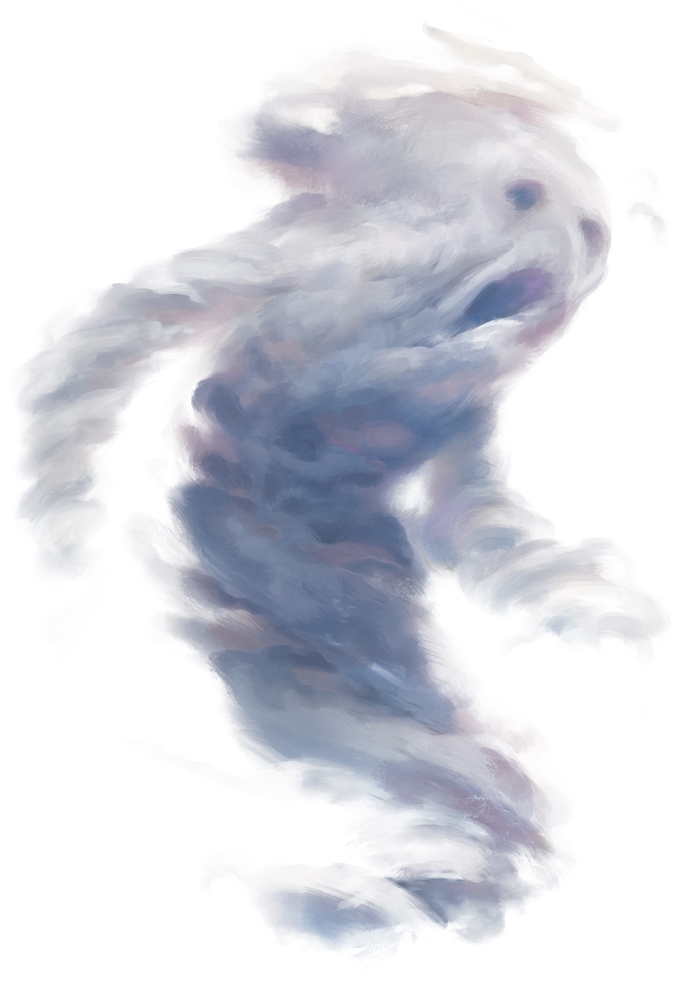
\includegraphics[width = 0.3\textwidth]{temporal-elemental}
	
	\emph{Temporal Elemental}
\end{center}